\subsection{Research design}
The Database Market that sells personal data is accessible through \url{http://d
atabase6e2t4yvdsrbw3qq6votzyfzspaso7sjga2tchx6tov23nsid.onion/} inside the
anonymous Tor network. The dataset provided by teacher Juha Nurmi captures web
pages of stolen credential information between November 2021 and June 2022.
The dataset can be downloaded from \url{https://mega.nz/folder/aJwVyIYJ#9SWh-Z3-
TpPfjHZeFxbeew}. In addition, I manually takes sorts of screenshots of the
marketplace, which needs to register a free account for authentication.

The provided dataset is an archive of 33,896 JSON files, 400 MB of raw size. Each
JSON file is represented as the following fields as shown in \autoref{fig:original_json}:

\begin{itemize}
    \item \emph{url}: URL address of webpage.
    \item \emph{text}: Text of the webpage.
    \item \emph{time-stamp}: Data collection date.
\end{itemize}

\begin{figure}
    \centering
    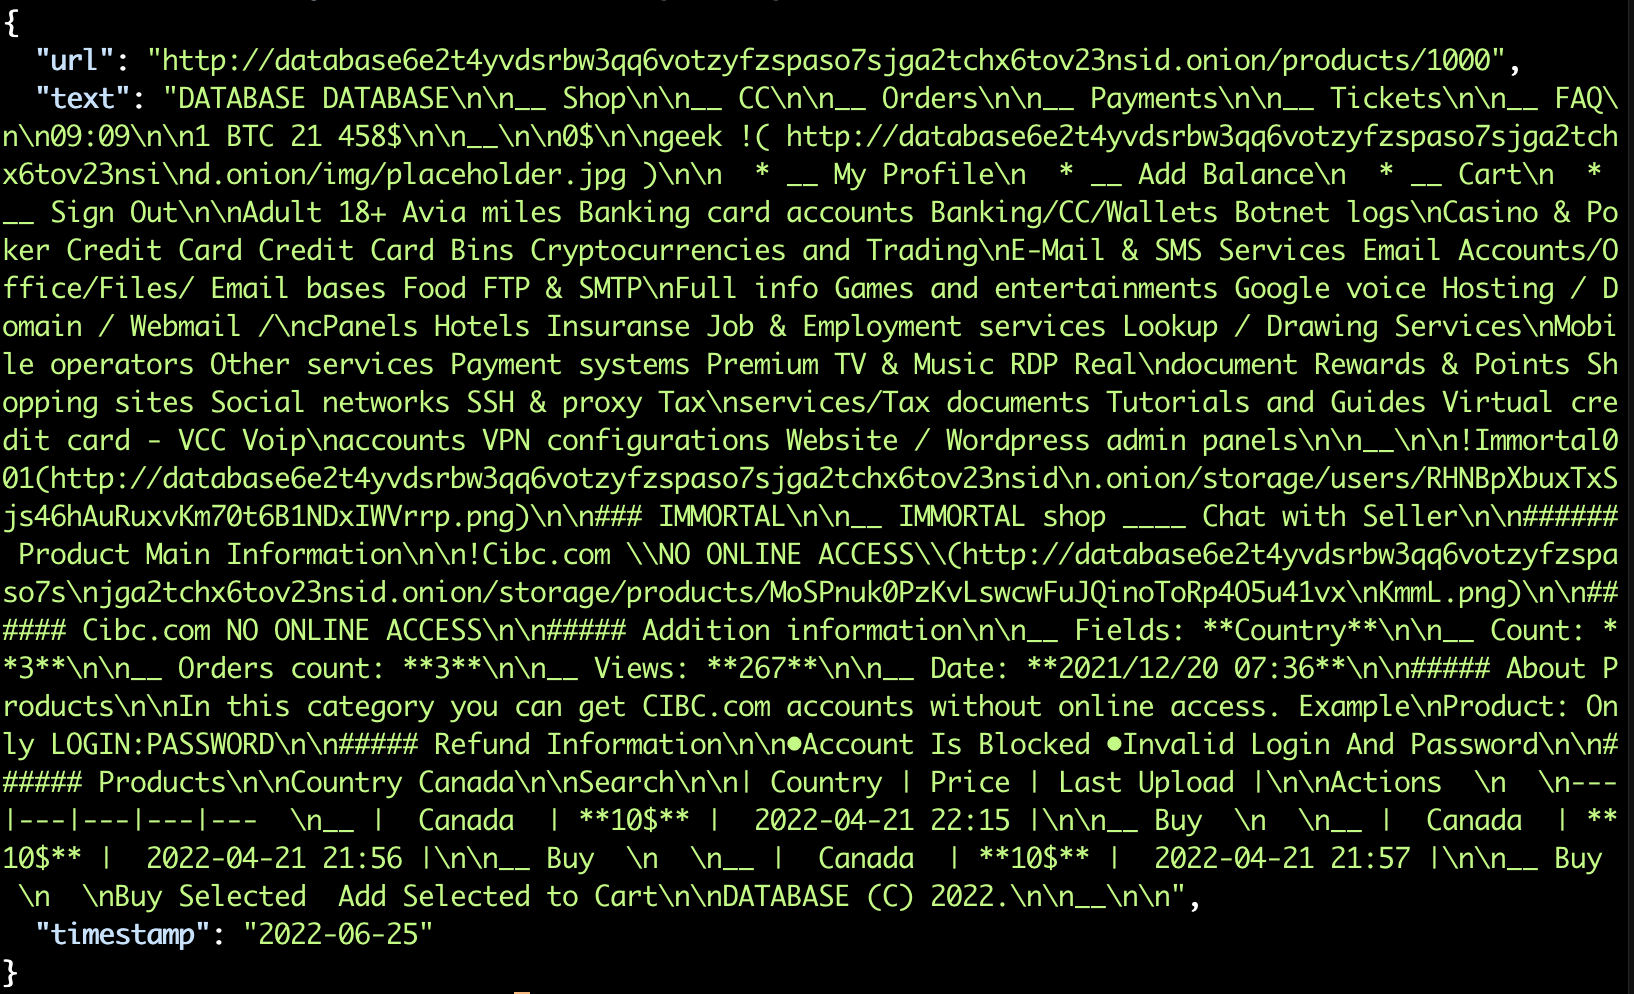
\includegraphics[width=\textwidth,height=\textheight,keepaspectratio]
    {orginal_json.png}
    \caption{An example JSON file from the provided dataset by Juha.}\label{fig:original_json}
\end{figure}

In order to achieve more insights of credentials for sale, I extracted from the \emph{text}
field of the original JSON files into several key fields storing into a single JSON file.
\autoref{fig:custom_json} is an example of an entry, where I assigned the following fields.

\begin{itemize}
    \item \emph{id}: ID of product.
    \item \emph{time-stamp}: Data collection date.
    \item \emph{seller}: Username of seller.
    \item \emph{product}: Name of product.
    \item \emph{prices}: Prices of items.
    \item \emph{dates}: Item uploaded date.
\end{itemize}

\begin{figure}
    \centering
    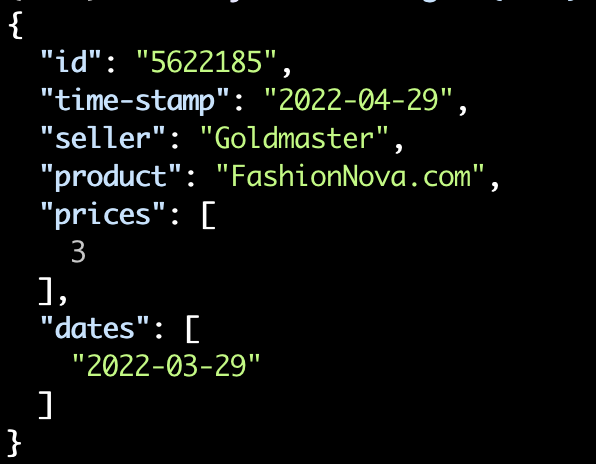
\includegraphics[width=\textwidth,height=\textheight,keepaspectratio]
    {customized_json.png}
    \caption{A example JSON entry from my customized dataset}\label{fig:custom_json}
\end{figure}

The datasets are under CC BY 4.0 license: You are free to copy, share, redistribute,
remix, transform, and build upon the material for any purpose, even commercially.
You must give attribution and appropriate credit. Follow the terms: \url{https:/
creativecommons.org/licenses/by/4.0/}.
In order to replicate my result, please do the following steps:

\begin{itemize}
    \item Access the original dataset provided by Juha Nurmi at \url{https://
    mega.nz/folder/aJwVyIYJ#}.
    \item Download \emph{database.tar.gz} (7 MB) and follow the instructions
    in \emph{README.md}.
    \item Check \emph{sha256sum}: \textbf{5a5f2cb4feb7fee597b0a26b1dc2fb33b1f
    9cae639e995a89663198bcfa76f1a}.
    \item Extract the compressed dataset (tar -xf database.tar.gz).
    \item 33,896 JSON files are generated in the destination folder.
    \item Clone the GitHub repo \url{https://github.com/ancuongnguyen07/Database
    _Market.git} and follow the comprehensive \emph{README.md} document.
\end{itemize}
